\documentclass[12pt,a4paper]{article}

\usepackage{parskip}
\usepackage[total={210mm,297mm}, left=20mm, right=20mm, top=20mm, bottom=20mm]{geometry}

\usepackage[utf8]{inputenc}
\usepackage[ngerman]{babel}%ngerman, french, italian
\usepackage{amsmath, amsthm, amssymb}
\usepackage{mathtools}%DeclarePairedDelimiter

\usepackage{graphicx}

\begingroup %parskip and amsthm fix
\makeatletter
   \@for\theoremstyle:=definition,remark,plain\do{%
     \expandafter\g@addto@macro\csname th@\theoremstyle\endcsname{%
        \addtolength\thm@preskip\parskip
     }%
   }
\endgroup

\theoremstyle{plain}
\newtheorem{thm}{Theorem}[section]
\newtheorem{satz}[thm]{Satz}
\newtheorem{lem}[thm]{Lemma}
\newtheorem{cor}[thm]{Korollar}
\newtheorem{alg}[thm]{Algorithmus}
\newtheorem{bsp}{Beispiel}

\theoremstyle{definition}
\newtheorem{defn}{Definition}[section]

\renewcommand{\phi}{\varphi} %kleines Phi
\newcommand{\nequiv}{\not \equiv}

\DeclareMathOperator{\ggT}{ggT}
\DeclareMathOperator{\kgV}{kgV}
\DeclareMathOperator{\ppcm}{ppcm}
\DeclareMathOperator{\pgcd}{pgcd}
\DeclareMathOperator{\ord}{ord}

\DeclarePairedDelimiter\abs{\lvert}{\rvert}
\DeclarePairedDelimiter\floor{\lfloor}{\rfloor}
\DeclarePairedDelimiter\frack{\{}{\}}

\renewcommand{\div}{\, | \,}
\newcommand{\ndiv}{\mathopen{\mathchoice{\not{|}\,}{\not{|}\,}{\!\not{\:|}}{\not{|}}}}
\newcommand{\R}{\mathbb{R}}
\newcommand{\N}{\mathbb{N}}
\newcommand{\Z}{\mathbb{Z}}

\begin{document}

\thispagestyle{empty}

\begin{center}
\Huge{\textbf{Finalrunde 2014 - Musterlösung}}\\ [0.7cm]
\large{15. März 2014}\\ [1.5cm]
\end{center}

\begin{itemize}
\item[\textbf{1.}]
Da $s$ die Spiegelung von $AB$ an $AC$ ist, gilt $\angle BAC=\angle CAH$. $ABCD$ ist ein Sehnenviereck, also gilt nach dem Peripheriewinkelsatz $\angle BAC=\angle BDC$. Zusammen folgt daraus $\angle CAH=\angle BDC$, folglich ist $AGDH$ ein Sehnenviereck.\\
Sei $E$ ein Punkt auf $t$ wie unten abgebildet. Nun folgt unter Verwendung des Tangentenwinkelsatzes:\\
\[\angle ECD= \angle CAD=\angle GHC\]
Somit ist $GH$ parallel zu $t$.\qed
\begin{center}
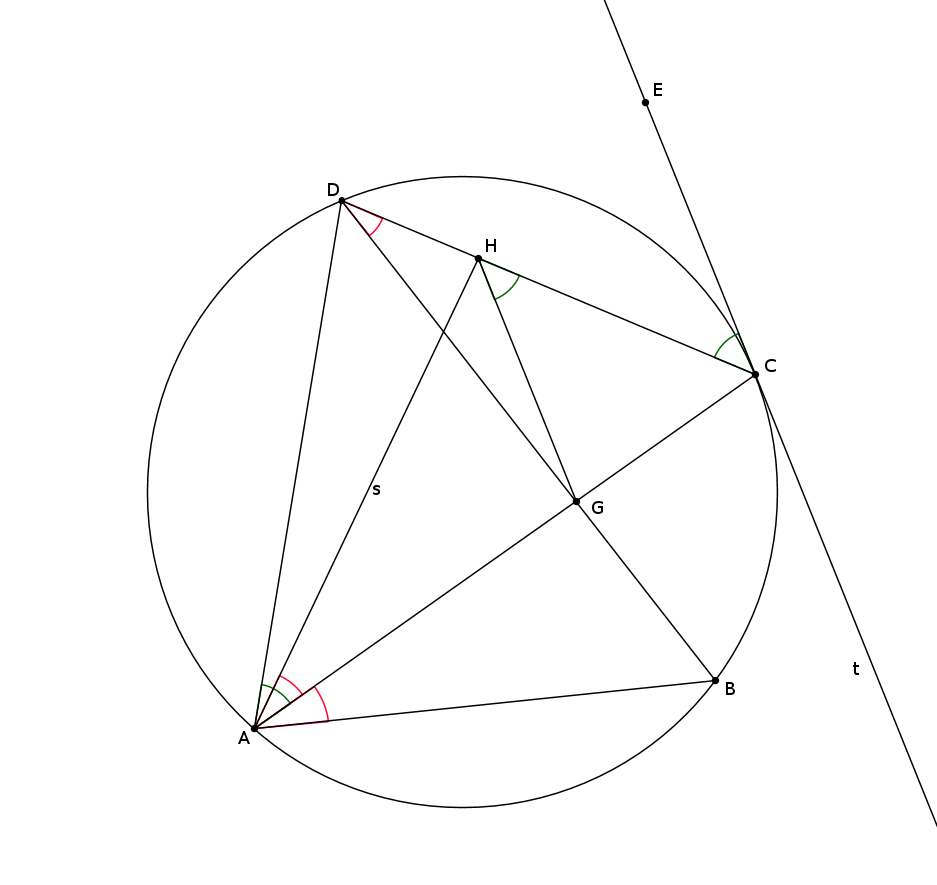
\includegraphics{Finalrunde14_1.png}
\end{center}


\item[\textbf{2.}]
Si on écrit $d=\pgcd(a,b)$ alors il existe $x,y\in\N$ tels que $a=dx$ et $b=dy$ avec $\pgcd(x,y)=1$. De plus avec ces notations $\ppcm(a,b) = xyd$ et il faut donc montrer que c'est un carré.
En substituant on obtient \[d^3xy(x-y) \div d^3 (x^3 + y^3)  + d^2 xy\] et donc on a aussi 
\begin{equation}\label{bla}
dxy(x-y)\div d(x^3 + y^3) + xy.
\end{equation}
Comme $x$ divise le côté gauche, on a que $x\div dx^3 + dy^3 + xy$ et ainsi $x\div dy^3$ et finalement $x\div d$ car $x$ et $y$ sont premiers entre eux. De manière analogue $y\div d$. En utilisant le fait que $\pgcd(x,y)=1$ encore une fois, on obtient que $xy\div d$. On peut aussi observer que le côté gauche de l'expression (\ref{bla}) est divisible par $d$ et donc $d\div xy$. Ainsi $d=xy$ et \[\ppcm(a,b) = xyd = (xy)^2\]
ce qui termine la preuve.\qed


\item[\textbf{3.}]
Wenn wir $x=0$ in die Funktionalgleichung einsetzen, bekommen wir $2f(0)=f(0)f(y)+yf(0)+0$. Umformen führt zu $(2-f(y)-y)f(0)=0$. Dies heisst, dass einer der beiden Faktoren null ist.
Die erste Möglichkeit liefert $f(y)=2-y$. Einsetzen zeigt, dass diese Funktion tatsächlich eine Lösung ist.

Die zweite Möglichkeit führt zu $f(0)=0$. Nun setzen wir $y=0$ in die ursprüngliche Gleichung ein. Daraus bekommen wir $f(x^2)=xf(x)$. Also gilt auch $xf(x)=f(x^2)=f((-x)^2)=-xf(-x)$. Aus dieser Gleichung folgern wir, dass die Funktion ungerade ist, denn wenn $x\neq0$, dann können wir $x$ aus der Gleichung kürzen und bekommen $f(x)=-f(-x)$. Wenn $x=0$, dann gilt $f(0)=0=-f(-0)$.\\
Nun setzen wir in der Aufgabenstellung $y=-x$. Dies führt zu $f(x^2)+f(-x^2)=f(x)f(-x)-xf(x)+xf(0)$. Da die Funktion ungerade ist, können wir $f(-z)$ mit $-f(z)$ ersetzen. Ausserdem gilt $f(0)=0$. Damit ergibt sich $f(x^2)-f(x^2)=-f(x)f(x)-xf(x)$, also $0=-f(x)^2-xf(x)$. Ausklammern führt zu $f(x)(f(x)+x)=0$. Dies heisst, dass einer der beiden Faktoren null ist.\\
Jetzt haben wir drei Möglichkeiten: $f(x)=0$, $f(x)=-x$ und Funktionen, die zwischen diesen beiden Funktionen springen. Einsetzen der ersten beiden Möglichkeiten ergibt, dass beide Lösungen sind. \\
Nun schliessen wir noch aus, dass es eine Lösungsfunktion gibt, die springt. Es gilt entweder $f(1)=-1$ oder $f(1)=0$. Der erste Fall führt mit Einsetzen von $x=1$ zu $f(1^2)+f(y)=f(1)f(y)+yf(1)+f(1+y)$.  Dies ist äquivalent zu $-1+f(y)=-f(y)-y+f(1+y)$. Also gilt $f(1+y)=-1+y-2f(y)$. Wenn nun für ein beliebiges $y$ gilt, dass $f(y)=0$, dann folgern wir $f(1+y)=-1+y$. Da wir nur zwischen den beiden oben genannten Funktionen springen dürfen, gilt $-1+y=0$ oder $-1+y=-1-y$, also $y=1$ oder $y=0$. Der erste Fall kann nicht eintreffen, da wir annehmen, dass $f(1)=-1$, der zweite Fall führt nicht zu Springlösungen, da $f(0)=0$ für beide Funktionen gilt.
Wenn $f(1)=0$ ist und wir wiederum $x=1$ einsetzen , bekommen wir $f(1^2)+f(y)=f(1)f(y)+yf(1)+f(1+y)$, also $f(1+y)=f(y)$. Dies ist nur der Fall, wenn für alle $y$ gilt, dass $f(y)=0$.\\
Man könnte Springlösungen auch ausschliessen, indem man für $f(xy)$ und $f(x+y)$ jeweils die Fälle durchtestet, also insgesamt vier Möglichkeiten ausrechnet.

Also hat die Funktionalgleichung die Lösungen $f(x)=2-x$, $f(x)=0$ und $f(x)=-x$.\qed


\item[\textbf{4.}]
Alle Paare $(a,b)$ mit $a\div b$ oder $b\div a$ sind gültige Paare.
Eine Konstruktionsmöglichkeit ist: 
ObdA $a<b$. Wir überdecken die Ebene mit $a \times b$-Rechtecken und verschieben jeweils Rechtecke eine Zeile weiter unten jeweils um $a$ Felder nach rechts. Jedes Rechteck färben wir gleich.\\
Man sieht leicht dass nun alle $a \times b$-Rechtecke alle Farben haben.
Nun gilt aber auch für zwei Felder gleicher Farbe dass wenn sie in vertikaler Richtung näher als $b$ sind, dann haben sie horizontalen Abstand mind. $a$. Also kommt keine Farbe in einem $b \times a$-Rechteck zwei mal vor, also muss jede Farbe genau einmal vorkommen.

Für alle andern Paare ist keine Färbung möglich:

\textit{Variante 1:}

Nehmen wir an wir haben eine gültige Färbung.
Wir betrachten ein Rechteck $a \times b$ und ObdA können wir annehmnen $a<b$ $a \ndiv b$ also $b=a \cdot k+r$ mit $0<r<a$.
Jetzt können wir die ganze Ebene neu färben indem wir alle Farben der ersten Zeile des Rechtecks mit einer neuen Farbe $c_1$ färben und dasselbe für jede andere Zeile des Rechtecks mit Farben $c_2, c_3... c_a$. Den Rest der Ebene färben wir so dass alle Felder die die selbe alte Farbe haben auch die selbe neue Farbe erhalten.
Nun muss in jedem Rechteck das wir platzieren können jede neue Farbe genau b mal vorkommen.
Wenn wir aber nun unser Rechteck eine Zeile nach unten verschieben wissen wir, dass dort auch wieder alle Farben b mal vorkommen müssen, woraus folgt, dass in der untersten Zeile alle Farben gleich $c_1$ sein müssen. Jetzt schieben wir unser rechteck immer eine Zeile weiter nach unten und folgern dass die Farben vorgegeben sind und jede Zeile der Reihe nach gleich gefärbt ist (zumindest unterhalb des Rechtecks).
Wenn wir aber nun das hochgestellte rechteck $a \times b$ betrachten erhalten wir dass die anzahl felder mit $c_1$ gefärbt ist $a\cdot k+1 > b$, was ein Widerspruch ist. \qed

\textit{Variante 2:}

Sei ObdA $a<b$ und $a \ndiv b$ also $b=a \cdot k+r$ mit $0<r<a$. Wir betrachten ein Feld der grösse $b \times (b+1)$. Betrachten wir die Farbe $c$ ganz oben links. Da wir das ganze rechteck mit ($k+1$) vielen $b \times a$-Rechtecken überdeckt werden kann, folgt dass $c$ höchstens $k+1$ mal vorkommen darf.
Nun können wir zwei $a \times b$ Rechtecke oben links und oben rechts plazieren woraus folgt, falls $c$ ganz oben links ist, muss c auch noch einmal in der Spalte ganz rechts vorkommen (jedes der beiden Rechtecke muss c genau einmal enthalten).
Nun betrachten wir aber das Feld $b \times (b+1)$ ohne die Spalte ganz links und die Spalte ganz rechts. Dieses ist $b \times b-1$. Aber da $(b-1) = a \cdot k+r -1 \ge a \cdot k$ können wir mind. $k$ hochgestellte Rechtecke überlappungsfrei hineinplatzieren und da es in jedem Rechteck c mind. ein mal vorkommen muss, folgt dass im Feld $c$ mindestens $k$ mal vorkommt. Also hat es im grossen Feld mind. $(k+2)$ mal $c$ $\rightarrow$ Widerspruch. \qed


\item[\textbf{5.}]
Wir verwenden Induktion nach $n$. Die Aussage stimmt offensichtlich für $n=1$.
Nehme nun an, die Aussage stimme für alle Zahlen kleiner als $n$ und schreibe $n=p^kn'$,
wobei $p$ ein Primteiler von $n$ ist und $(p,n')=1$. Nun gilt

\[2^n=\sum_{d\div n}a_d = \sum_{d\div p^{k-1}n'} a_d + \sum_{d\div n'}a_{p^kd} =2^{p^{k-1}n'}+\sum_{d\div n'}a_{p^kd}.\]

Nach Induktionsannahme ist jeder Summand von $\sum_{d\div n'}a_{p^kd}$ ausser $a_n$ durch $p^k$ teilbar.
Weiter gilt $p^k\div 2^n - 2^{p^{k-1}n'} = 2^{p^{k-1}n'}(2^{n'\phi(p^k)}-1)$ für alle ungeraden Primzahlen nach dem 
Satz von Euler-Fermat und für $p=2$ direkt. Daraus folgt, dass $p^k$ auch $a_n$ teilt, für jeden Primteiler $p$ von $n$
und somit schliesslich auch $n\div a_n$.\qed

\item[\textbf{6.}]
Wir machen zuerst folgende Beobachtung:
\[\frac{3-b}{a+1}=\frac{2+(1-b)}{a+1}=\frac{2+a+c}{a+1}=1+\frac{c+1}{a+1}\]
Nun folgt mit AM-GM:
\begin{align*}
\frac{3-b}{a+1}+\frac{a+1}{b+1}+\frac{b+1}{c+1}&=1+\frac{c+1}{a+1}+\frac{a+1}{b+1}+\frac{b+1}{c+1}\\
&\geq1+3\sqrt[3]{\frac{c+1}{a+1}\cdot\frac{a+1}{b+1}\cdot\frac{b+1}{c+1}}\\
&=4
\end{align*}
\qedhere

\item[\textbf{7.}]
\textbf{Schritt 1:} Wir zeigen zuerst, dass wir endlich viele Routenänderungen vornehmen können, sodass danach alle Fähren Santa Marta anfahren. Wir sagen dabei, dass eine Stadt mit Santa Marta \textit{verbunden} ist, falls sie eine Nachbarstadt von Santa Marta ist oder eine Fähre zwischen dieser Stadt und Santa Marta verkehrt.\\
Wir starten bei Santa Marta und gehen im Uhrzeigersinn um den See herum. Wenn alle Städte mit Santa Marta verbunden sind, sind wir fertig. Ansonsten bezeichnen wir mit $B$ die erste Stadt, welche nicht mit Santa Marta verbunden ist. Sei $A$ die letzte Stadt vor $B$. $A$ ist nach Definition von $B$ mit Santa Marta verbunden. Weiter sei $C$ die nächste Stadt nach $B$, welche wieder mit Santa Marta verbunden ist. Wir können uns sicher sein, dass eine solche Stadt $C$ existiert, da Santa Marta eine Nachbarstadt im Gegenuhrzeigersinn besitzt.\\
Wir wissen aus der Geometrie, dass ein $n$-Eck durch $n-3$ sich nicht schneidende Diagonalen in $n-2$ Dreiecke unterteilt wird. Für uns bedeutet dies also, dass zwischen $A$ und $C$ eine Fähre verkehrt. Wir ändern nun die Route dieser Fähre, sodass diese Fähre danach zwischen Santa Marta und einer Stadt $D$ verkehrt, wobei $D$ eine Stadt ist, die im Uhrzeigersinn zwischen $A$ und $C$ liegt. $D$ kann dabei dieselbe Stadt wie $B$ sein, kann aber auch eine andere Stadt sein.\\
Wir bemerken, dass nach dieser Routenänderung die Anzahl Fähren, die Santa Marta anfahren, um 1 grösser geworden ist. Wenn wir obiges Vorgehen also genügend oft wiederholen, fahren schlussendlich alle Fähren Santa Marta an.\\
\begin{center}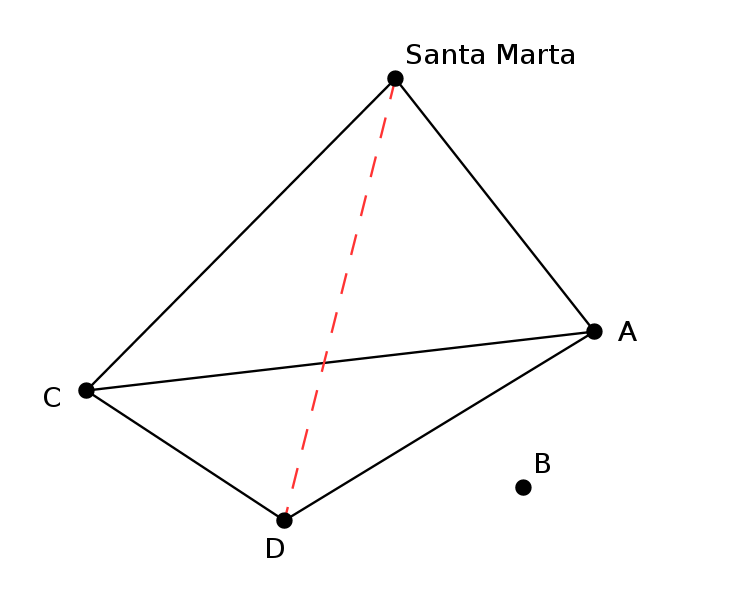
\includegraphics{Finalrunde14_7-1.png}\end{center}
\textbf{Schritt 2:} Seien $F_1$ und $F_2$ zwei Fähren, sodass $F_1$ zwischen Santa Marta und einer Stadt $S$ verkehrt, $F_2$ zwischen Santa Marta und einer Stadt $T$ verkehrt und $T$ direkt nach $S$ am See liegt. Wir zeigen nun, dass wir einige Routenänderungen vornehmen können, sodass danach $F_1$ und $F_2$ ihre Routen vertauscht haben.\\
Sei $R$ die letzte Stadt vor $S$ und $U$ die nächste Stadt nach $T$ im Uhrzeigersinn. $R$, $S$, $T$ und $U$ liegen also in dieser Reihenfolge im Uhrzeigersinn am See und sind alle mit Santa Marta verbunden.\\
Wir können nun folgende Routenänderungen vornehmen:
\begin{itemize}
\item Ändere die Route von $F_2$ von Santa Marta - T zu S-U.
\item Ändere die Route von $F_1$ von Santa Marta - S zu R-U.
\item Ändere die Route von $F_2$ von S-U zu R-T.
\item Ändere die Route von $F_1$ von R-U zu Santa Marta - T.
\item Ändere die Route von $F_2$ von R-T zu Santa Marta - S.
\end{itemize}
Nach diesen Routenänderungen haben wir die Routen von $F_1$ und $F_2$ vertauscht.\\
\begin{center}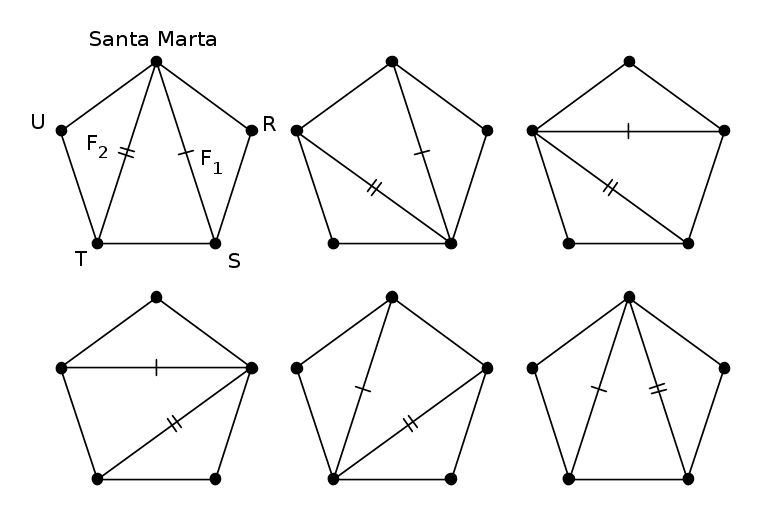
\includegraphics{Finalrunde14_7-2.png}\end{center}
\textbf{Schritt 3:} Nach Schritt 1 können wir mit Schritt 2 die Routen der Fähren so vertauschen, dass die grüne Autofähre zwischen Santa Marta und Kapstadt verkehrt, und dann sind wir fertig.\qed

\item[\textbf{8.}]
Seien $B'$ und $C'$ die Fusspunkte der Höhen $h_b$ und $h_c$. Die Dreiecke $ABB'$ und $AC'C$ beinhalten jeweils den Winkel $\angle BAC$ und einen rechten Winkel, folglich sind diese Dreiecke ähnlich. $M$ und $N$ sind die Mittelpunkte von einander entsprechenden Seiten, folglich sind auch die Dreiecke $ABM$ und $ANC$ sowie die Dreiecke $AMB'$ und $AC'N$ ähnlich. Insbesondere gilt also $\angle B'MA=\angle ANC'$. Hieraus folgt sofort, dass $MNPQ$ ein Sehnenviereck ist und wir sind fertig.\qed
\begin{center}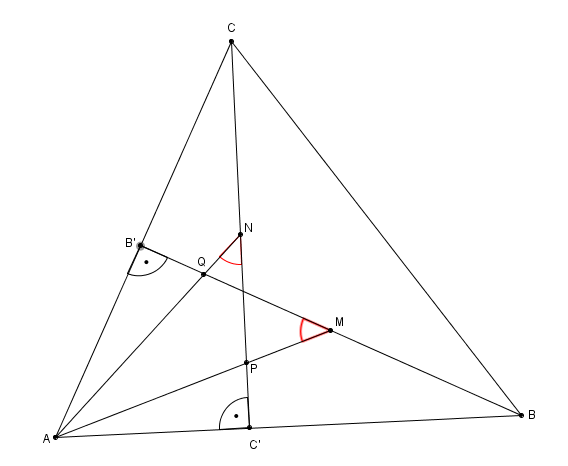
\includegraphics{Finalrunde14_8.PNG}\end{center}

\item[\textbf{9.}]
\textbf{1. Lösung:} Nehme an die Folge $a_n$ wird irgendwann periodisch. Sei $T$ die Periodenlänge und $S$ die kleinste Zahl ab der die Folge periodisch ist. Wähle $k$ sodass $T^{2k}>S$ und eine Primzahl $p> T^{2k}$. Sei $d_n$ die Anzahl Teiler von $n$. Sei $m$ nicht durch $p$ teilbar. Es gibt $d_m$ Teiler von $mp$, die durch $p$ teilbar sind und $a_m$ Teiler von $mp$, die nicht durch $p$ teilbar und grösser als $2014$ sind. Es folgt
\begin{align*}
a_{mp}\equiv d_m+a_m \ (2)
\end{align*} 
Setze $m=T^{2k}$, welches eine Quadratzahl ist und somit $d_m \equiv 1 \ (2)$. Es folgt $a_{mp} \equiv 1 + a_m \ (2)$. Da aber $T | mp$ und $T | m$ ist dies ein Widerspruch zur Periodizät. \qed

%2. Lösung: Seien $S$ und $T$ wie oben. Sei $z$ das Produkt aller Primzahlen, die kleiner als $2014$ sind. 

\textbf{2. Lösung:} Dirichlets krasses Theorem aus der Zahlentheorie besagt, dass wenn $ggT(m,T)=1$, dann gibt es unendlich viel Primzahlen, die gleich $m$ modulo $T$ sind. Seien $S$ und $T$ wie oben. Aus Dirichlets Theorem folgt, dass es eine Primzahl $p>S$ gibt mit $p \equiv 1 \ (T)$. Es gilt $a_p =1$ und $a_{p^2}=0$ und $T| p^2-p$, Widerspruch zur Periodizität.\qed

\item[\textbf{10.}]
\textbf{1. Lösung:}\\
Soient $M$ le point d'intersection de $BD$ et de $TC$ et $I$ le point d'intersection de $DT$ avec $AB$. Les points $M,B$ et $D$ sont alignés, on peut donc appliquer Meneleaüs au triangle $CIT$ et on obtient :\\
\begin{equation}
\left|\frac{TM}{MC}\cdot\frac{CB}{BI}\cdot\frac{ID}{DT}\right|=1
\end{equation}
Soit $\alpha =\angle BAT$. Par le théorème de l'angle tangent, $\angle BTC = \alpha$. Comme $AB$ est un diamètre, $\angle ABT = 90^\circ -\angle BAT = 90^\circ - \alpha$. Donc $\angle ITB = 90^\circ-\angle IBT = \alpha$.\\
De plus, $TC$ est parallèle à $AD$, donc $\angle TCA = 90^\circ -2\alpha = \angle CAD$.\\
On a donc $\angle DAT = 90^\circ-2\alpha+\alpha=90^\circ-\alpha=\angle ATD$ et donc le triangle $ ATD$ est isocèle en $D$. Donc $AD=DT$.\\
Soit $B_h$ la projection de $B$ sur $TC$.\\
Le triangle $BB_hC$ est semblable au triangle $AID$ (3 angles en commun). Donc :
\[
\frac{CB}{BB_h}=\frac{AD}{ID}=\frac{DT}{ID}
\]
De même, le triangle $TB_hB$ est semblable au triangle $TBI$. Donc :
\[
\frac{BB_h}{BI}=\frac{BT}{BT}=1 \rightarrow BB_h=BI
\]
Au final, $\frac{CB}{BI}=\frac{DT}{ID}$ et injecté dans la première équation, on a $TM=MC$. \qed
\begin{center}
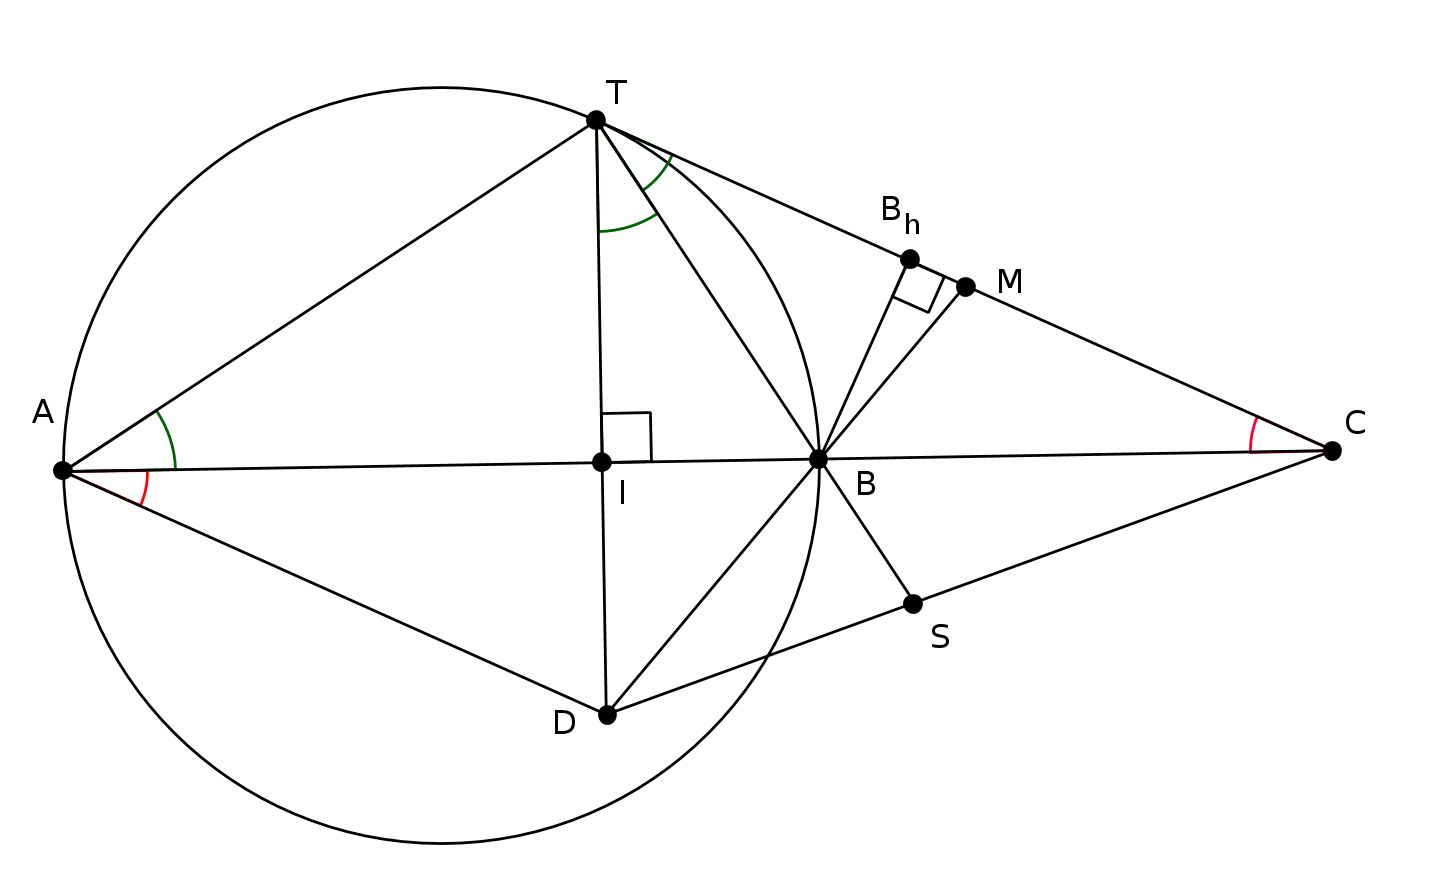
\includegraphics{Finalrunde14_10.png}
\end{center}
\textbf{2. Lösung:}\\
Sei $S$ der Schnittpunkt von $DC$ und $TB$. Weiter sei $M$ der Schnittpunkt von $DB$ und $TC$ und $I$ der Schnittpunkt von $TD$ und $AC$. Die Geraden $DM$, $TS$ und $IC$ schneiden sich in $B$, also gilt nach Ceva:
\[\frac{DS}{SC}\cdot\frac{CM}{MT}\cdot\frac{TI}{ID}=1\]
Wenn wir nun zeigen können, dass $\frac{DS}{SC}\cdot\frac{TI}{ID}=1$ gilt, sind wir fertig.\\
Es gilt $\angle ATB=90^\circ=\angle BIT$, also sind die Dreiecke $ABT$ und $IBT$ ähnlich. Hieraus folgt, dass $\angle ITB=\angle BAT=\angle BTC$ gilt, wobei wir im letzten Schritt den Tangentenwinkelsatz verwendet haben. $TS$ is also die Winkelhalbierende im Dreieck $TDC$ und es gilt:
\[\frac{DS}{SC}=\frac{TD}{TC}\]
Da $AD$ parallel zu $TC$ ist, gilt $\angle DAI=\angle TCI$ und die Dreiecke $TIC$ und $ADI$ sind ähnlich. Somit folgt:
\[\frac{TI}{ID}=\frac{TC}{AD}\]
Sei $\alpha=\angle ITB=\angle BTC=\angle BAT$. Mit der Innenwinkelsumme im Dreieck $ICT$ erhalten wir $\angle DAC=\angle TCI=90^\circ-2\alpha$. Es folgt:
\[\angle ATI=\angle 90^\circ-\angle DTB=90^\circ-\alpha=90^\circ-2\alpha+\alpha=\angle DAI+\angle IAT=\angle DAT\]
Das Dreieck $ADT$ ist also gleichschenklig und es gilt $AD=DT$. Insgesamt folgt daraus:
\[\frac{DS}{SC}\cdot\frac{TI}{ID}=\frac{TD}{TC}\cdot\frac{TC}{AD}=\frac{TD}{AD}=1\]
Damit ist alles gezeigt.\qed
\end{itemize}
\end{document}